\documentclass[a4paper,12pt]{article}
\usepackage{amsmath, amssymb, graphicx}
\graphicspath{ {D:/Library/Meteorology/Notes_tex/baroins} }

\DeclareMathAlphabet{\mathcal}{OMS}{cmsy}{m}{n}
\SetMathAlphabet{\mathcal}{bold}{OMS}{cmsy}{b}{n}
\newcommand{\bigO}{\mathcal{O}}


\begin{document}

\title{\vspace{-4.0cm}Baroclinic Instability}
\author{Ian Beckley
\\University of Wisconsin-Madison}

\date{2 Dec. 2020}

\maketitle

\subsection*{Outline}

\begin{enumerate}
	\item Sloping convection and the release of APE
	\item The Eady problem (1949), Rossby height, short wave cut-offs
	\item The Charney problem (1947), long wave cut-off, instability diagram
	\item Synoptic structure of growing baroclinic waves
	\item Observed momentum and heat fluxes
	\item Baroclinic wave life cycles - energy conversion
\end{enumerate}

Readings: Holton Ch. 6, Gill Ch. 12, 13; James (1994)

\subsection*{Sloping convection and the release of APE}

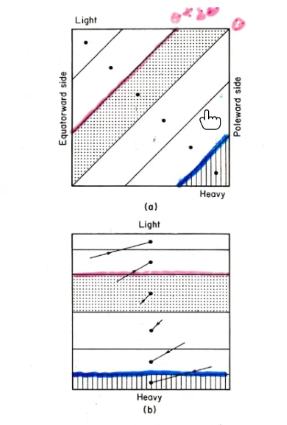
\includegraphics[width=\textwidth]{1}
Figure a. demonstrates the sloping isentropes associated with the equatorward temperature gradient. Each dot represents the center of mass associated with each 'slab' of atmosphere. The change in entropy accross an isobar ensures the prescence of available potential temperature.  Figure b. represents the release of available potential energy and the lowering of the center of mass.

\subsubsection*{Baroclinic Instabilty}

\begin{itemize}
	\item Baroclinic horizontal temp. gradient $\frac{\partial u}{\partial z} = -\frac{g}{f}\frac{1}{\theta}\frac{\partial \theta}{\partial y}$
	\item "The existence of a jet requires available potential energy"
	\item Slantwise convection allows PE $\rightarrow$ KE
	\item Wavelength of maximum growth $\sim 4000 \text{ km}$
	\item $\beta$ effect is stabilizing
\end{itemize}

\subsubsection*{Slantwise Convection}
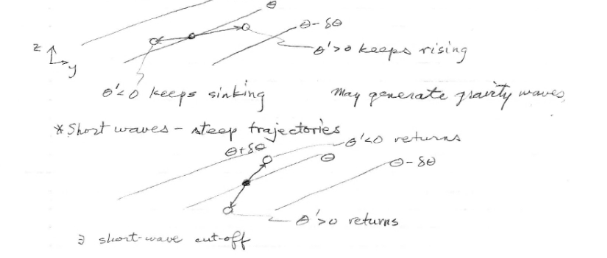
\includegraphics[width=\textwidth]{2}
Note that static stability is positive everywhere. If you shift a warm parcel northward, $\theta' > \theta$ and the parcel will continue to rise (reverse for a southward parcel movement); this is an unstable situation. 

For steep parcel trajectories, a parcel pushed upward will experience $\theta'<\theta$ and sink back; this is a stable situation. This is known as the short-wave cut-off.

Clearly parcels can be inertially unstable only if their convective slant/slope is less than that of the local isentropes.

\subsection*{The Eady Problem (Gill 13.3)}
\begin{enumerate}
	\item Boussinesq: $\rho$ constant except for sloping buoyancy
	\item Baroclinic: $\frac{\partial u}{\partial z} = -\frac{g}{f}\frac{1}{\theta}\frac{\partial \theta}{\partial y}$
	\item Rigid lids with $w' = 0$: Clearly the upper B.C. is not reflective of the real world
	\item $\beta = 0$: Also not reflective of the real world
\end{enumerate}

Begin with

\begin{align*}
q = \nabla^2 \psi f + \frac{f^2}{N^2}\frac{\partial^2\psi}{\partial z^2}
\end{align*}

Linearize QGPV eqn $\frac{dq}{dt} = 0$

\begin{align*}
(\frac{\partial}{\partial t} + \overline{u} \frac{\partial}{\partial x})(\nabla^2 \psi f + \frac{f^2}{N^2}\frac{\partial^2\psi}{\partial z^2}) = 0
\end{align*}

Let's assume $\psi = \text{Re}\left[\psi(z)e^{i(kx-\omega t)}\right]$ so that $\psi = \psi_r + i\psi_i$ and $\omega = \omega_r + i\omega_i$. It follows that $\frac{2\pi}{\omega_i}$ proposes a timescale for baroclinic, unstable growth.

 Let's define the vertical structure function,

\begin{align*}
-k^2 \psi + \frac{f^2}{N^2}\frac{\partial^2}{\partial z^2} \psi = 0 \text{ w/ canceled} -i(\omega - \overline{u}k)e^{ik}\\
\psi(z) = A\sinh{\alpha z} + B \cosh{\alpha z}\\
\alpha = \frac{Nk}{f} = \frac{1}{H_R}
\end{align*}

Where $H_R$ is the 'Rossby height"

\begin{align*}
\boxed{H_R = \frac{f}{Nk}}
\end{align*}

which is a measure of e-folding scale of the decay of a potential vorticity perturbation on either lid. 

Eady's solution (with work included in Holton and Gill)

\begin{align*}
(\omega - k\overline{u})^2 = (kH\frac{\partial \overline{u}}{\partial z})^2\left[\frac{1}{4} + \frac{1}{(H\alpha)^2} - \frac{\coth{H\alpha}}{H\alpha}\right]
\end{align*}

\begin{itemize}
	\item a). $\omega_i \neq 0 \rightarrow \text{ wave growth } \propto \frac{\partial u}{\partial z}$
	\item a). $\omega_r = k\overline k\overline{u}$ drifting at the steering flow speed
	\item b). $\frac{NHk}{f} \approx 1.6$ or $L_x = \frac{2\pi}{1.6}\frac{N}{f}H$
	\item b). Maximum growth $L_x \sim 2400 \text{ km}$ for scale height $H = 8 \text{ km}$ (However, this is commonly observed...)
	\item c). $\frac{HNk}{f} > 2.3$ or $L_x < \frac{2\pi H N}{2.3 f}$, shortwave cutoff $\sim 1600 \text{ km}$
	\item c). static stability stabilizes shortwaves (slanting convection is too steep)
	\item $w'$ required to keep T hydrostatic during relative vorticity advection...
	\item $-\overline{u} \frac{\partial}{\partial x} \nabla^2 \psi \sim -\frac{u\psi}{L_x} \rightarrow$ large for shortwaves $\rightarrow$ large vertical motion, steep slopes
	\item d.) $\omega_i \sim \frac{\partial u}{\partial z} \sim \frac{30 \text{ m s}^{-1}}{10 \text { km}}$; $\frac{2\pi}{\omega_i} = \tau_i \sim$ 2 days for growth by a factor of $e$. 
	\item d.) in the oceans, more like $\tau_i \sim 100 \text{ days}$
\end{itemize}

\subsection*{Charney Problem}

Charney included $\beta$ such that waves propagate westward relative to mean flow (west to east).

The long wave cut-off is 

\begin{align*}
|-\beta v| > |-v \cdot \nabla\zeta|
\end{align*}

where planetary vorticity advection is greater than relative vorticity advection. Recall

\begin{align*}
\frac{\partial \zeta}{\partial t} = -\vec{V_g} \cdot \nabla \zeta - \beta v_g - f\nabla \cdot \vec{V}
\end{align*}

which, for one example, demonstrates how a dominant planetary vorticity term forces positive vorticity spin-up upshear of a long-wave positive vorticity anomaly. Continuing with this example, in order to 'create' a positive PV anomaly to the west one must cool the layer to achieve lower heights aloft. Ascent is required to cool this layer and the required convergence at the surface will 'kill' the surface high pressure (recall westward tilt of anomalies with height). The impact of this is such that surface P patterns weaken, temperature advections stop, and $\beta$ effectively works to make all waves stable when vertical shear is weak.

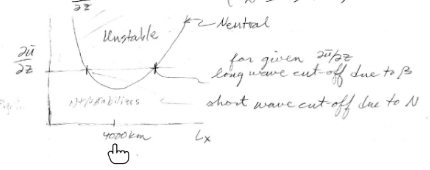
\includegraphics[width= \textwidth]{4}

\subsubsection*{Caveats}
\begin{itemize}
	\item Latent Heating
	\item Barotropic Instability 
	\item Surface Friction (Ekman Pumping)
	\item Wave-wave interactions
\end{itemize}

\subsubsection*{Ocean}
\begin{itemize}
	\item Eddies are produced near strong currents ($\frac{\partial u}{\partial z}$ or $\nabla T$)
	\item $\tau \sim 10-30 \text{ days}$ with $L \sim 10-100 \text{ km}$
	\item $\vec{V} \sim \vec{V_g} \sim 10 \text{ cm s}^{-1}$
	\item $c_x \sim -5 \text{ cm s}^{-1}$ which is against the stream! 
	\item $|h'| \sim 10 \text{ cm}$
\end{itemize}

\subsubsection*{Eady summary}
\begin{itemize}
	\item $f$-plane: meaning no $\beta$ effect (not Rossby waves)
	\item Rigid upper boundary
	\item warm axis is 21 degrees ahead of surface low
	\item $L_x$ set by the lid seperation
\end{itemize}

\subsubsection*{Charney summary}
\begin{itemize}
	\item $\beta$ retained
	\item warm axis 41 degrees ahead of low
	\item Steering level control
	\item $L_x$ and $L_y$ set by $\beta$
\end{itemize}

The Eady baroclinic growth rate is given as

\begin{align*}
\omega_i = .31 \frac{f}{N}\frac{\partial u}{\partial z}
\end{align*}




\end{document}